\documentclass[12pt,a4paper]{report}
\usepackage{url}
\usepackage{listings}
\usepackage{supertabular}
\usepackage{hhline}
\usepackage{array}
\usepackage{color}
\usepackage{tikz}
\usepackage[dvips, bookmarks, colorlinks=false, pdfborder={0 0 0}, pdftitle={Code Coverage in Functional Concurrent Languages},
 pdfauthor={Shayan Najd Javadipour}, pdfsubject={Project Report}, pdfkeywords={}]{hyperref}
\setcounter{secnumdepth}{0}
\makeatletter
\newcommand\arraybslash{\let\\\@arraycr}
\makeatother
\lstset{language=erlang}
\title{Code Coverage in Functional Concurrent Languages}
\author{Shayan Najd Javadipour}
\date{Fall 2011}
\begin{document}
\maketitle
\addcontentsline{toc}{chapter}{Abstract}
\begin{abstract}
Code coverage is a measure indicating how much of the actual code is exercised in the process of testing. However, code coverage metrics are mostly defined with the focus on imperative languages. When the target is a functional language, to be more effective, these metrics should be redefined.

In this project, we studied existing code coverage metrics and then we defined an equivalent criterion specialized for functional languages. Based on this metric, we developed a tool, named \emph{FCover}, measuring code coverage in a functional concurrent language, namely Erlang. We designed the tool in a way that its output can be used to define a stopping function for automated property based test case generation.

\emph{FCover} first extracts the abstract syntax tree (AST) of the input Erlang code and then it generates an instrumented code by transforming the AST to a semantically equivalent AST. This instrumentation is used to log the data useful for measuring the code coverage. In the last step, the logged data is post-processed to generate the final coverage information.  

In this report, first we describe the existing concepts related to code coverage and at the end of each section, we discuss our interpretation and implementation. Later in the second chapter, we discuss our approach for measuring code coverage in Erlang code including the necessary code transformations for the instrumentation. We also describe the application of this coverage information in automated property based test case generation.
\end{abstract}
\addcontentsline{toc}{chapter}{Table of Contents}
\tableofcontents
\chapter{Code Coverage in Theory}
\newpage
\section{Code Coverage}
Code coverage is a measure indicating how much of the actual code is exercised in the process of testing. Code coverage criteria are used as a measure of test adequacy.\cite{Zhu:1997:SUT:267580.267590}

In this project, we studied existing code coverage metrics and then we defined an equivalent criterion specialized for functional languages. This equivalent criterion arguably provides a stronger notion of code coverage and it is comparably efficient. In the following sections, we discuss this equivalent metric in more detail.

\section{Statement Coverage}
Statement coverage---also closely named \emph{node coverage}, \emph{line coverage}, \emph{segment coverage} \cite{Ntafos:1988:CST:630792.631017}, \emph{basic block coverage} and \emph{C1} \cite{beizer2002software}---is defined as: 

``A set $P$ of execution paths, satisfies the statement coverage criterion if and only if for all nodes $n$ in the flow graph, there is at least one path $p$ in $P$ such that node $n$ is on the path $p$.''\cite{Zhu:1997:SUT:267580.267590}

There are several different interpretations for ``node in the flow graph'' in the above mentioned definition such as:

\begin{enumerate}
 \item Statements (statement coverage)
 \item A single line of code (line coverage)
 \item A single basic block; block of code with no branching (basic block coverage)
 \item Expressions 
 \item etc
\end{enumerate}

Often, control flow graphs (CFG) only model the execution flow of programs without considering the exception flows. Exception flow is an execution flow initiated by exceptions, errors or exit signals. For example, the term $throw$ $"error"$  branches the main execution flow by generating an exception. A complete CFG includes both the normal execution flows and the exception flows. Based on this definition of the CFG, we can redefine node coverage which is arguably more precise.

In this project, we define a special version of node coverage targeting functional languages. Since almost everything in a functional language is an expression, comprehensive definition of ``node in the flow graph'' would be ``expression in a program''. 

The CFG starts with the \emph{source node} and ends with the \emph{sink node}. Neither of them have any semantical operation.

For representing the complete CFG in a functional program, the CFG should include exception flows. For this purpose, we add one extra virtual node, a fork, exactly before each node and it has an edge to the exception node. This virtual node represents the branching when an exception is generated. The exception node is a normal node representing the execution flow of the program when the exception is generated. It has an edge to the \emph{sink node} or to the initial node of an exception handling structure. 

For example, the expression $1/X$ is represented as three nodes in the CFG:
\begin{enumerate}
 \item Virtual node: a fork with the condition $X\neq0$. It has an edge labeled $True$ to the normal node and an edge labeled $False$ to the exception node.
 \item Normal node: a node that represents the expression when there is no exception. It has an edge to the node that represents the next expression in the execution flow
 \item Exception node: is a node in the exception flow that represents the generation of the exception; for example, $throw$ $"Division by zero"$. It has an edge to either \emph{sink node} or to the initial node of the exception handling structure (EHS)
\end{enumerate}
 \begin{center}
\begin{figure}
\centering
 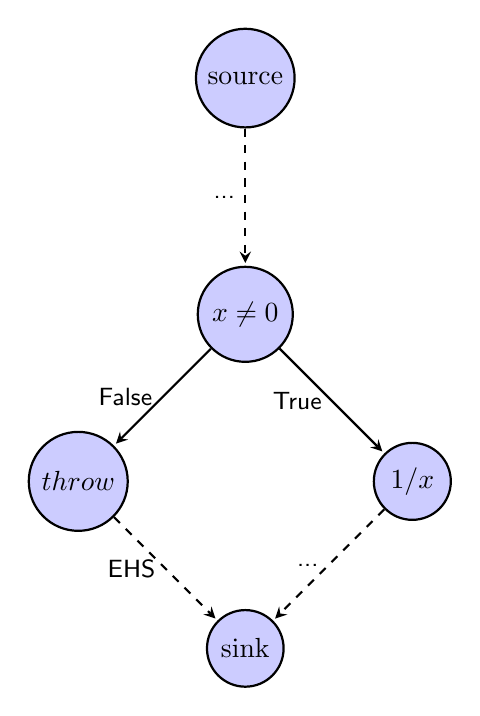
\begin{tikzpicture}[->,>=stealth,shorten >=1pt,auto,node distance=3cm,
  thick,every node/.style={circle,fill=blue!20,draw}]

  \node (in) {source};
  \node (vn) [below of=in]   {$x \neq 0$};
  \node (nn) [below right of=vn]   {$1 / x$ };
  \node (en) [below left of=vn]   {$throw$};
  \node (sn) [below right of=en]   {sink};

  \path[dashed,every node/.style={font=\sffamily\small}]     
    (in) edge node [left] {...} (vn);

  \path[every node/.style={font=\sffamily\small}]
    (vn) edge node [left] {True}  (nn)        
         edge node [left] {False} (en);
  \path[dashed,every node/.style={font=\sffamily\small}]     
    (nn) edge node [left] {...}  (sn)  
    (en) edge node [left] {EHS}  (sn);  
      
\end{tikzpicture}
\caption{a CFG with virtual node}
\label{fig:virtualnode}
\end{figure}
 \end{center}

Here we can define two types of node coverage based on the complete graph. The first one considers the exception node as a normal node that should be covered in testing and the weaker form that does not include exception nodes in the coverage measurements. The virtual nodes are ignored in both types. Our implementation is of the first type, covering all the nodes including the exception nodes.

In a functional language, every expression should return a value and there is no looping. Therefore, the CFG of a functional language is acyclic. In fact, there is looping in functional languages. For example, recursion is a way to simulate looping. But the main point is that in unit testing we focus on one single function. In that function, we consider function calls---even self calls---as abstract expressions. These abstract expressions either terminate and return a value, or do not terminate at all. In the case of nontermination we can consider a new exception flow but usually they can be merged with the existing exception flow. If we merge the two, a nontermination is equivalent to the case that the callee returns an exception. 

We also implemented some form of optimization. We cut the CFG on the specific cut-points and that would break the CFG into smaller parts; the distinct set of connected nodes between the two consecutive cut-points. Each of these smaller parts form a tree\footnote{Binary tree, since decisions are Boolean}.

In a complete CFG, we define cut-points by:  

\begin{enumerate}
 \item Immediately after the \emph{source node} is a cut-point
 \item Immediately before the \emph{sink node} is a cut-point
 \item Immediately after the first node in the beginning of each branch, including the exceptional branches\footnote{Each exceptional branch has only one node which is the exception node.} 
\end{enumerate}

To achieve full node coverage, we need to make sure that all the leaves of these smaller parts are visited. That is because each leaf in these trees can uniquely define a path in the tree and when the execution flow reaches the beginning of the path, all the expressions in the path are executed.
 
\begin{center} 
\begin{figure}
\centering
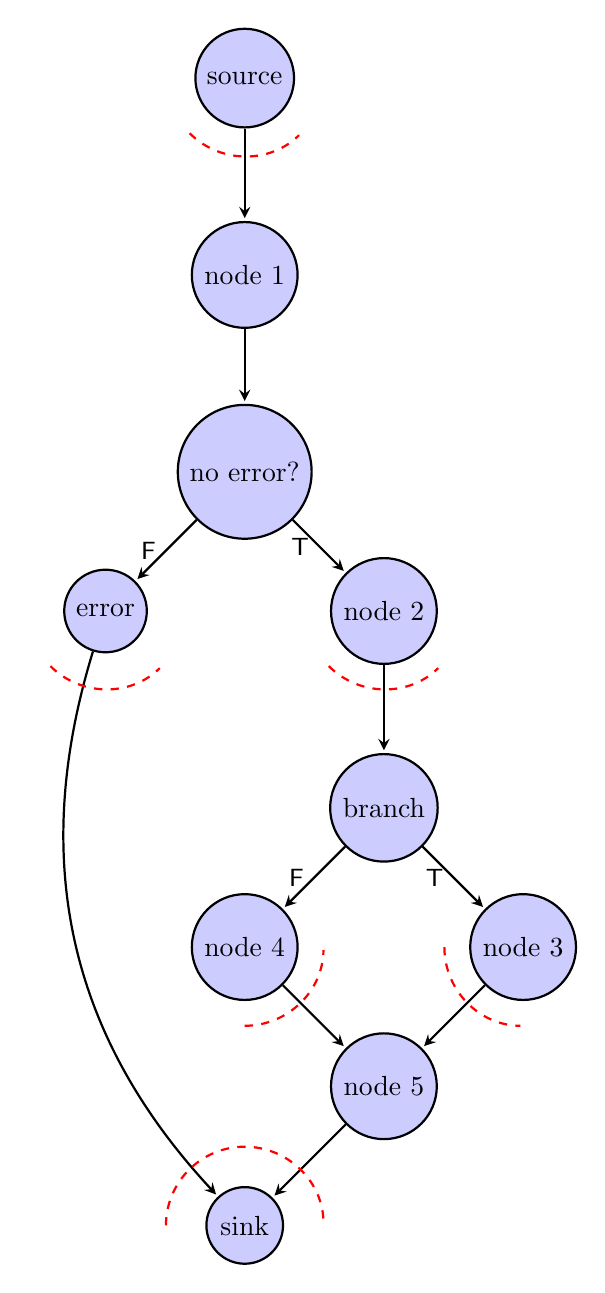
\begin{tikzpicture}[->,>=stealth,shorten >=1pt,auto,node distance=25mm,scale=0.50,
  thick,main node/.style={circle,fill=blue!20,draw},hidden node/.style={fill=white,draw=none,text=white}]

  \node[main node] (in) {source};
  \node[main node] (n1) [below of=in]   {node 1};  
  \node[main node] (vn) [below of=n1]   {no error?};
  \node[main node] (n2) [below right of=vn]   {node 2};
  \node[main node] (bn) [below of=n2]   {branch};
  \node[main node] (nt) [below right of=bn]   {node 3};
  \node[main node] (nf) [below left of=bn]   {node 4};
  \node[main node] (n5) [below right of=nf]   {node 5};
  \node[main node] (en) [below left of=vn]   {error};
  \node[main node] (sn) [below left of=n5]   {sink}; 
 

 \path[every node/.style={font=\sffamily\small}]
    (in) edge node [left] {} (n1)
    (n1)  edge node [left] {} (vn)
    (vn)  edge node [left] {T} (n2)
          edge node [left] {F} (en)
    (n2)  edge node [left] {} (bn)
    (bn)  edge node [left] {T} (nt)
          edge node [left] {F} (nf)
    (nt)  edge node [left] {} (n5)
    (nf)  edge node [left] {} (n5)
    (n5)  edge node [left] {} (sn)
    (en)  edge [bend right] node [left] {} (sn);  
 \draw[-,red,dashed] (nf)++(0,-2) arc (270:360:2cm);
 \draw[-,red,dashed] (nt)++(-2,0) arc (180:270:2cm);
 \draw[-,red,dashed] (in)++(-1.4,-1.4) arc (225:315:2cm);  
 \draw[-,red,dashed] (n2)++(-1.4,-1.4) arc (225:315:2cm);  
 \draw[-,red,dashed] (en)++(-1.4,-1.4) arc (225:315:2cm);
 \draw[-,red,dashed] (sn)++(-2,0) arc (180:0:2cm);      
\end{tikzpicture}
\caption{a sample CFG and cut-points}
\label{fig:cutpoints}
\end{figure}
\end{center}

In summary, in our implementation we monitor the execution of:

\begin{enumerate}
 \item the exception nodes
 \item the fist node after the \emph{source node}
 \item the nodes at the beginning of each branch
\end{enumerate}

\section{Decision Coverage}
Along with \emph{all-edges coverage}, \emph{C2} and \emph{decision-decision-path testing}; \emph{decision coverage} and \emph{branch coverage} are closely related code coverage metrics.

Branch coverage is defined as:

``A set $P$ of execution paths satisfies the branch coverage criterion if and only if for all edges $e$ in the flow graph,there is at least one path $p$ in $P$ such that $p$ contains the edge $e$.''\cite{Zhu:1997:SUT:267580.267590}

Decision coverage is defined as:

``Decision Coverage - Every point of entry and exit in the program has been invoked at least once and every decision in the program has taken on all possible outcomes at least once.''\cite{cast-10}

And \emph{decision} is defined as:

``A Boolean expression composed of conditions and zero or more Boolean operators. A decision without a Boolean operator is a condition. If a condition appears more than once in a decision, each occurrence is a distinct condition.''\cite{cast-10}

Where \emph{condition} is:

``A Boolean expression containing no Boolean operators.''\cite{cast-10}

In functional languages, beside Boolean expressions\footnote{They are often called guards.}, pattern matchings are used to form conditional clauses. To have a more comprehensive coverage metric, patterns should be considered a form of Boolean expressions. In Fcover, we transform a pattern $p$ of variable $X$ to a Boolean expression $match(p,X)$. Since patterns are not often first-class entities in functional languages, $match$ is a meta-level function.

In the definition of decision coverage all the Boolean expressions are included while branch coverage considers only the ones immediately before each fork.

The complete CFG of a functional program has a special property: if you visit all the nodes you have visited all the edges. Therefore, for such CFG, node coverage and branch coverage are equivalent. 

FCover provides the specified node coverage; consequently, it also provides branch coverage.

In FCover, we add a monitor on top of the Boolean expressions in each conditional clause. Monitors, or loggers, observe and log the value of the Boolean expression at runtime. So later on, after preprocessing, we can check from the logged data whether all of these Boolean expressions were evaluated to both $True$ and $False$. However, there are difficulties in implementing decision coverage for dynamic type languages since ``Boolean expression'' is not defined. For Erlang, in our view, it is satisfactory to cover only the Boolean expressions inside control flow statements.

 
\section{Condition Coverage}
\emph{Condition coverage}, also closely referred to as \emph{predicate coverage}, is defined as follows:

``Condition coverage requires that each condition in a decision take on all possible outcomes at least once (...), but does not require that the decision take on all possible outcomes at least once. In this case, for the decision ($A$ or $B$) test cases ($TF$) and ($FT$) meet the coverage criterion, but do not cause the decision to take on all possible outcomes. As with decision coverage, a minimum of two tests cases is required for each decision.''\cite{KellyJ.:2001:PTM:886632}

As mentioned in the previous section, patterns should be considered a form of Boolean expression. Each sub-pattern of a pattern forms a separate condition, in a similar way that subexpressions of a Boolean expression do. 

In this work, we decompose a decision into conditions and observe their values at execution time. Condition coverage can be computed by post-processing this logged data. It is done by comparing the logged values of each condition with the expected permutations. However, due to the difficulties mentioned in the previous section, we limit ourselves to the conditions in each conditional clause. 

\section{Multiple Condition Coverage}
\emph{Multiple condition coverage} is defined as follows:

``A test set $T$ is said to be adequate according to the multiple-condition-coverage criterion if, for every condition $C$, which consists of atomic predicates $(p1, p2,  . . .  , pn)$, and all the possible combinations $(b1, b2,  . . .  , bn)$ of their truth values, there is at least one test case in $T$ such that the value of $pi$ equals $bi$, $i = 1, 2,  .  .  .  , n$.'' \cite{Zhu:1997:SUT:267580.267590}

In our terminology, a ``condition'' is a decision and ``predicate'' is a condition. 

\emph{Multiple condition coverage} grows exponentially in respect to the number of conditions in a decision, but it is easy to calculate. In practice, the number of conditions in a decision is often so low that it does not affect performance.

In this project, we calculate this metric by post-processing the logged data. It is done by verifying, for each decision, whether all the possible combinations in the truth table exist. This coverage metric is also extended to include patterns.

\section{Condition / Decision Coverage}
C/D Coverage is a mixture of condition coverage and decision coverage. It is defined as:

``Condition/decision coverage combines the requirements for decision coverage with those for condition coverage. That is, there must be sufficient test cases to toggle the decision outcome between $True$ and $False$ and to toggle each condition value between $True$ and $False$. Hence, a minimum of two test cases are necessary for each decision. Using the example $(A or B)$, test cases $(TT)$ and $(FF)$ would meet the coverage requirement. However, these two tests do not distinguish the correct expression $(A or B)$ from the expression $A$ or from the expression $B$ or from the expression $(A and B)$.''\cite{KellyJ.:2001:PTM:886632} 

In FCover, C/D coverage is done by post-processing the logged data in the same way as decision coverage and condition coverage. This coverage metric is also extended to include patterns.

\section{Modified Condition / Decision Coverage (MCDC)}
This criterion is part of the standard ``DO-178B'', and states:

``Every point of entry and exit in the program has been invoked at least once, every condition in a decision in the program has taken all possible outcomes at least once, every decision in the program has taken all possible outcomes at least once, and each condition in a decision has been shown to independently affect that decision's outcome. A condition is shown to independently affect a decision's outcome by varying just that condition while holding fixed all other possible conditions.''\cite{cast-10}

There are three important points in the implementation of MC/DC coverage:

\begin{enumerate}
 \item How to handle shortcut logical operators
 \item How to handle multiple/nested conditional control flows
 \item How to handle repeated condition in a decision, also tautologies/contradictions
\end{enumerate}
 
Moreover, this method should be extended to include patterns.

There are different ways to handle shortcut logical operators in functional programs:

\begin{enumerate}
 \item Treating all the shortcut operators the same as their non-shortcut equivalents
 \item Considering separate internal decisions for the operands\cite{DO-248B} 
 \item Keeping conditions constant if they are not executed due to a shortcut operator\cite{chilenski1994applicability}
\end{enumerate}
 
Since decisions have no side effects in Erlang and errors/exceptions are equivalent to the Boolean value $False$, we can ignore the shortcut behavior of the operators and compute coverage assuming they are normal Boolean operators.  
 
For measuring the MCDC coverage, in this project, an exhaustive algorithm is implemented to calculate whether a test suite passes the coverage. The input of the algorithm is the logged data. In this project we treat shortcut operators as normal operators and in case of chronological dependency, we interpret ``logically undefined'' as logical $False$. A condition named \emph{child} is chronologically dependent on the condition named \emph{parent} where \emph{child} is meaningless if \emph{parent} does not hold. For example, ``$element(1,X)$'' in the following code requires ``$is\_tuple(X)$'' to hold:

\begin{lstlisting}
foo(X)->
    if is_tuple(X) andalso element(1,X)==2 -> ok;
       true -> false
end.
\end{lstlisting} 

In case of multiple and nested control flow statements, the problem is how to include contexts in calculations. By contexts, we can determine whether a condition is repeated and in that case, what is its value. Having this information, we can compute coverage treating the repeated condition as a Boolean constant with the value extracted from the context (environment). A simpler solution is to consider each nested decision as a separate decision with extra conditions indicating their contextual preconditions. For example, in ``if'' with multiple guards, the second guard is evaluated only if the first guard does not hold. In that case, we add negation of the first guard condition with shortcut operator ``andAlso'' to the decision of the second guard.

It is possible that conditions are not completely independent from each other and there are also chances of repeated conditions. Two solutions to this problem are defined as follows:

``Unique Cause MCDC: A Form of MCDC which allows for masking to be used only in the case of coupled conditions to show a condition’s independence. Otherwise, only the condition of interest is allowed to change between the two truth vectors of the independence pair. The condition’s change is (generally) the unique cause of the change in the expression’s outcome, hence the name.''\cite{chilenski2001investigation}

``Masking MCDC: A form of MCDC that allows all possible forms of masking to be used to show a condition’s independence.''\cite{chilenski2001investigation}

Where ``masking'' is defined as:

``The process of setting the RHS (LHS) operand of an operator to a value such that changing the LHS (RHS) operand of that operator does not change the value of the operator. For an AND operator, masking of the RHS (LHS) can be achieved by holding the LHS (RHS) False.  Recall from Boolean algebra that $X AND False = False AND X = False$ no matter what the value of X is. For an OR operator, masking of the RHS (LHS) can be achieved by holding the LHS (RHS) True. Recall from Boolean algebra that $X OR True = True OR X = True$ no matter what the value of $X$ is.'' \cite{chilenski2001investigation}

In this project, after observing the values of the conditions in each decision at the execution time, we compute MCDC coverage by post-processing the logged data. With our algorithm we can find conditions that do not even have one pair of test cases to determine their independence. Hence, we can identify tautologies; contradictions, decision independent from conditions; and dummy conditions, conditions that their value does not change decisions. There are several optimized algorithms in the literature that can generate test cases for the complete MCDC coverage.

\section{Path Coverage}
Path coverage is a complex, yet powerful, form of code coverage. Because of the implementation complexities and practical difficulties, there are several weaker variations of this coverage that are more useful in practice. 

Path Coverage is defined as follows:

``A set $P$ of execution paths satisfies the path coverage criterion if and only if $P$ contains all execution paths from the begin node to the end node in the flow graph.''\cite{Zhu:1997:SUT:267580.267590}

Path coverage is not implemented in this project due to its complexity and inefficiency. 

Bellow follows a list of some of the coverage metrics based on path coverage:
\subsection{Basis Path Coverage}
In this metric, execution paths that are in the same class and only differ in the number of loops (recursions), are identified. Then, complete basis path coverage demands testing at least one path in each class.

\subsection{JJ-Path Coverage (LCSAJ Coverage)}
This criterion determines if all jump to jump paths (LCSAJs) have been executed. 

LCSAJ can be defined as:

``An LCSAJ consists of a body of code through which the flow of control may proceed sequentially and which is terminated by a jump in the control flow. The hierarchy $TERi$ , $i = 1, 2, . . . ,n, . . .$ of criteria starts with statement coverage as the lowest level, followed by branch coverage as the next lowest level.''\cite{Zhu:1997:SUT:267580.267590}

\subsection{Data Flow Coverage}
It is a form of path coverage that only includes the sub-paths from variable bindings to the subsequent references of the variables.
 
\subsection{Predicate Coverage}
It is defined as:
``We say that predicate coverage has been achieved if all possible combinations of truth values corresponding to the selected path have been explored under some test. Predicate coverage is clearly stronger than branch coverage. If all possible combinations of all predicates under all interpretations are covered, we have the equivalent of total path testing. Just as there are hierarchies of path testing based on path segment link lengths, we can construct hierarchies based on different notions of predicate coverage.''\cite{beizer2002software}

\subsection{All-Definition Coverage}
The definition is as follows:
``A set P of execution paths satisfies the all-definitions criterion if and only if for all definition occurrences of a variable x such that there is a use of x which is feasibly reachable from the definition, there is at least one path p in P such that p includes a subpath through which the definition of x reaches some use occurrence of x.''\cite{Zhu:1997:SUT:267580.267590}

\subsection{All-Uses Coverage}
\emph{All-Uses Coverage} is described as:
``A set P of execution paths satisfies the all-uses criterion if and only if for all definition occurrences of a variable x and all use occurrences of x that the definition feasibly reaches, there is at least one path p in P such that p includes a subpath through which that definition reaches the use.''
\cite{Zhu:1997:SUT:267580.267590}

\subsection{All Definition-Use-Paths (All DU-Paths)}
The definition is as follows:
``A set P of execution paths satisfies the all-du-paths criterion if and only if for all definitions of a variable x and all paths q through which that definition reaches a use of x, there is at least one path p in P such that q is a subpath of p, and q is cycle-free or contains only simple cycles.''
\cite{Zhu:1997:SUT:267580.267590}

\subsection{N-Length Sub-path Coverage}
\emph{N-Length Sub-path Coverage} determines whether each path with length $N$ is executed.

\subsection{Required k-Tuples Criteria}
It is defined as:
``A set P of execution paths satisfies the required k-tuples criterion, $k > 1$, if and only if for all j-dr interactions L, $1 < j \leq k$, there is at least one path p in P such that p includes a subpath which is an interaction path for L.''\cite{Zhu:1997:SUT:267580.267590}

\section{Other Code Coverage Metrics}

\subsection{Function Coverage}
If all the functions or subroutines in the program are called, we achieve complete function coverage.
In this project we implement the general form of it, Entry/Exit Coverage.

\subsection{Entry/Exit Coverage}
If all the functions (or subroutines) in the program are called (entry) and return a value (exit), complete entry/exit coverage is achieved.
We add two observation points (logging points) to each function, one in the beginning and one in the exit. After execution of the test cases we can measure the coverage based on the logged data. 

\subsection{Call Coverage / Call Pair Coverage}
With the assumption that most bugs lie in the interfaces between code blocks, this method determines whether all the function calls have been executed.
In this project for each function call there is an exception node and normal node that should be covered. If there is no exception indicating that function cannot be called, $100\%$ call coverage is achieved, otherwise each of these exceptions reveal a function-call bug.

\subsection{Loop coverage (recursion coverage)}
This coverage metric determines whether each loop in the program has been executed zero, one or multiple times. In functional programs we can replace this coverage metric with ``Recursion Coverage''. Recursion coverage determines whether recursion happened zero, one or multiple times. In this project the recursion coverage can be achieved by searching the logged data to check if there are zero, one or multiple records of function-entry for the same function name.

\subsection{Relational Operator Coverage}
This metric measures whether every expression with comparison operators is tested with its boundary values.
This metric is not yet implemented in the tool.
 
\subsection{Table Coverage}
Table coverage indicates whether each entry in a particular array has been referenced.\cite{andersson2005automatic}
This metric is not implemented in the tool.

\subsection{Race Coverage}
Monitors the code at execution time and reports which parts of the code have been executed with multiple threads (processes). This information helps discovering race conditions. 
This tool does not support this metric.

\section{Object Code Related Coverages}
There are several metrics to check the quality of test cases at the object code level, in the compiler or directly after compilation of the code.
Since the tool works with high-level code, these metrics are not implemented.

\section{Fault Based Coverages}
There are several metrics determining the quality of test suites and their code coverage by adding some forms of error inside the code.
This tool does not support these metrics.

\chapter{Our Approach}
\newpage

\section{Coverage Information}
In FCover, raw coverage information is a list of program points and their corresponding information. Since later on we use the tool as a stop function, we collect special information for the different categories of program points to be able to identify identical test cases. Program points are relative positions inside a function tracked globally using a central state counter. During the AST transformation, the transformer requests a new program point from the counter and assigns it to the logger to embed it inside the augmented code. For example:

\begin{lstlisting}
fooFunc () -> 
      bar.  
\end{lstlisting}

Has multiple program points including:

\begin{enumerate}
 \item Function Entry
 \item Function Exit
 \item etc
\end{enumerate}
 
A path would be an ordered list of these logged tuples. For the above mentioned example, it would be something like:

\begin{lstlisting}
[ {ProcessID# , fooFunc, programPoint 1
    ,Line 2,{functionEntry}}
  ,...
  ,{ProcessID# , fooFunc, programPoint n
    ,Line 2,{functionExit}}]
\end{lstlisting}

The first part of each element is the $PID$ of the process executing the test case. The second part is the name of the function and the third is the relative program point in the function. The line number of the original code is in the fourth part. The fifth part contains some detailed information about each program point.   
 
\section{Code Transformation}
To be able to log required and useful information, we inject loggers to different parts of the original code. We transform the code, via AST transformation, into a semantically equivalent instrumented version. In the following sections, we list and discuss these transformations.

\subsection{Enclosing Errors}
In the section about statement coverage, we mentioned that our interpretation of node in the complete control flow graph includes branched execution flows due to errors and exceptions. To log information related to exceptions we wrap each error producing, or exception producing, language construct inside a block implemented by try-catch to log the exception information. Below follows a list of possible expressions\cite{ErlangAbstractSyntax} and indication of whether they generate errors at runtime if the arguments do not return exceptions (errors):

 
\begin{supertabular}{| p{13cm} | p{2cm} |} 
\hline
Expression Type
&
Possibility of Run\-Time Error
\\\hline
literal
&
No
\\\hline
P = E 
&
Yes
\\\hline
variable V 
&
No
\\\hline
tuple skeleton
\{E\_1, ..., E\_k\}
& 
No
\\\hline
empty\ list\ []
&
No
\\\hline
\ cons\ skeleton\ [E\_h\ {\textbar}\ E\_t]
&
No
\\\hline
binary\ constructor\ {\textless}{\textless}V\_1:Size\_1/TSL\_1,\ ...,\ V\_k:Size\_k/TSL\_k{\textgreater}{\textgreater}
&
Yes
\\\hline
E\_1\ Op\ E\_2,\ where\ Op\ is\ a\ binary\ operator
&
Yes
\\\hline
Op\ E\_0,\ where\ Op\ is\ a\ unary\ operator
&
Yes
\\\hline
\#Name\{Field\_1=E\_1,\ ...,\ Field\_k=E\_k\}
&
No
\\\hline
\ E\_0\#Name\{Field\_1=E\_1,\ ...,\ Field\_k=E\_k\}
&
Yes
\\\hline
\#Name.Field
&
No
\\\hline
E\_0\#Name.Field
&
Yes
\\\hline
catch\ E\_0
&
No
\\\hline
E\_0(E\_1,\ ...,\ E\_k)
&
No
\\\hline
E\_m:E\_0(E\_1,\ ...,\ E\_k)
&
Yes
\\\hline
list\ comprehension\ [E\_0\ {\textbar}{\textbar}\ W\_1,\ ...,\ W\_k],\ where each W\_i is a generator or a filter
&
 Yes
\\\hline
binary comprehension {\textless}{\textless}E\_0\ {\textbar}{\textbar}\ W\_1,\ ...,\ W\_k{\textgreater}{\textgreater}, where each W\_i is a generator or a filter
&
 Yes
\\\hline
 begin\ B\ end,\ where\ B\ is\ a\ body
&
 No
\\\hline
if\ Ic\_1\ ;\ ...\ ;\ Ic\_k\ end,\ where\ each\ Ic\_i\ is\ an\ if\ clause\ 
&
 Yes
\\\hline
case\ E\_0\ of\ Cc\_1\ ;\ ...\ ;\ Cc\_k\ end,\ where\ E\_0\ is\ an\ expression\ and\ each\ Cc\_i\ is\ a\ case\ clause\ 
&
 Yes
\\\hline
try\ B\ catch\ Tc\_1\ ;\ ...\ ;\ Tc\_k\ end,\ where\ B\ is\ a\ body\ and\ each\ Tc\_i\ is\ a\ catch\ clause
&
 No
\\\hline
try\ B\ of\ Cc\_1\ ;\ ...\ ;\ Cc\_k\ catch\ Tc\_1\ ;\ ...\ ;\ Tc\_n\ end,\ where\ B\ is\ a\ body,\ each\ Cc\_i\ is\ a\ case\ clause\ and\ each\ Tc\_j is\ a\ catch\ clause
&
 Yes
\\\hline
try\ B\ after\ A\ end,\ where\ B\ and\ A\ are\ bodies
&
No
\\\hline
try\ B\ of\ Cc\_1\ ;\ ...\ ;\ Cc\_k\ after\ A\ end,\ where\ B\ and\ A\ are\ a\ bodies\ and\ each\ Cc\_i\ is\ a\ case\ clause
&
Yes
\\\hline
try\ B\ catch\ Tc\_1\ ;\ ...\ ;\ Tc\_k\ after\ A\ end,\ where\ B\ and\ A\ are\ bodies\ and\ each\ Tc\_i\ is\ a\ catch\ clause\ 
&
No
\\\hline
try\ B\ of\ Cc\_1\ ;\ ...\ ;\ Cc\_k\ catch\ Tc\_1\ ;\ ...\ ;\ Tc\_n\ after\ A\ end,\ where\ B\ and\ A\ are\ a\ bodies,\ each\ Cc\_i\ is\ a\ case\ clause\ and\ each\ Tc\_j\ is\ a\ catch\ clause
&
Yes
\\\hline
receive\ Cc\_1\ ;\ ...\ ;\ Cc\_k\ end,\ where\ each\ Cc\_i\ is\ a\ case\ clause
&
No
\\\hline
receive\ Cc\_1\ ;\ ...\ ;\ Cc\_k\ after\ E\_0\ {}-{\textgreater}\ B\_t\ end,\ where\ each\ Cc\_i\ is\ a\ case\ clause,\ E\_0\ is\ an\ expression\ and\ B\_t\ is\ a\ body
&
Yes
\\\hline
fun\ Name\ /\ Arity
&
No
\\\hline
fun\ Module:Name/Arity
&
No
\\\hline
fun\ Fc\_1\ ;\ ...\ ;\ Fc\_k\ end\ where\ each\ Fc\_i\ is\ a\ function\ clause
&
No
\\\hline
query\ [E\_0\ {\textbar}{\textbar}\ W\_1,\ ...,\ W\_k]\ end,\ where\ each\ W\_i\ is\ a\ generator\ or\ a\ filter
&
We\ do\ not\ support
\\\hline
E\_0.Field,\ a\ Mnesia\ record\ access\ inside\ a\ query 
&
We\ do\ not\ support\ 
\\\hline
parenthesized\ expressions\ (\ E\_0\ )
&
No
\\\hline
\end{supertabular}
 
To wrap all the above mentioned constructs which may raise an exception, we use the same code block. An example of transformed code for expression $1 * 9$  at line $3$ of function $f$ would be:
 
\begin{lstlisting}
    try 
        1 * 9 
    catch
        exit:VarUnique2 ->
            rareLoggerName ! 
	      {self(), f, 2, 3, {exception}},
            exit(VarUnique2);
        error:VarUnique2 ->
            rareLoggerName ! 
	      {self(), f, 2, 3, {exception}},
            erlang:error(VarUnique2);
        VarUnique2 ->
            rareLoggerName !
	      {self(), f, 2, 3, {exception}},
            throw(VarUnique2)
    end.
\end{lstlisting}

The catch part has three cases, one for each possible category of exceptions. It first executes the expression and if there is no exception, it returns the value. If exceptions are generated, it catches them, logs them and re-throws them again. As mentioned before there is a central logger server named ``rareLoggerName'' that logs messages sent from different parts of the instrumented code. Here, the recorded message is ``exception''. 

\subsection{Function/Abstraction Transformation}
Functions are first transformed to a set of case clauses representing their pattern matching behaviors and then the case clause transformation is applied on the result of the first transformation. Also in the first transformation, we have to design a wildcard pattern to return the ``match\_failure'' error specific to the function instead of the case specific one. There are loggers at the beginning and at the end of the function body to log function entry and function exit. For example, function definition:

\begin{lstlisting}
   f([X])->X.
\end{lstlisting}

is first transformed into:

\begin{lstlisting}
f(XUnique1) ->
     begin
          ExpUnique_2 = {XUnique1},
           case ExpUnique_2 of
            {X} ->  X;
            _ -> erlang:error(function_clause)
          end
        end.
\end{lstlisting}

and then in the second stage, the case expression is transformed. In the first stage, the arguments of the function are all wrapped in a tuple, over which the pattern matching happens and a special clause is added to generate ``function match\_failure'' error instead of ``case match\_failure''.

\subsection{If Transformation}
Loggers are placed on top of the ``if'' structure to observe the value of the conditions in decisions. For example:

\begin{lstlisting}
if 
  X < 1 -> v1;
  X > 1 -> v2
end 
\end{lstlisting}

is transformed into an equivalent code of this pseudo-code:

\begin{lstlisting}
begin
  loggerForIfClause,
  loggerForIfClause,  
  if 
    X < 1 ->
	    loggerForClauseEntry
	    , v1;
    X > 1 ->
	    loggerForClauseEntry
	    , v2
  end
end 
\end{lstlisting}

The first logged message includes textual representation of the decision and its actual value. There is also another logger, in the beginning of the clause, logging clause entry. It is possible to have exceptions in the decision part of the control flow statements; an error case in Erlang is equal to $False$. Therefore, the actual transformation of:

\begin{lstlisting}
if 2 > 1 -> 1 end
\end{lstlisting}

would be:

\begin{lstlisting}
begin
  rareLoggerName !
    {self(), f, 2, 3,
	{"try 2 > 1 catch _:_ -> false end"
	  , try 	
		2 > 1 
	    catch 
		_:_ -> false 
	    end}},
  if 2 > 1 ->
      rareLoggerName ! {self(), f, 3,
	      3, {clauseEntry}}
      , 1
  end
end 
\end{lstlisting}

\subsection{Case Transformation}
For each case clause there is a logger on top of the case block to log the conditions in the decisions of each clause.
 
For example:
\begin{lstlisting}
case 1 of 
  1 -> v1
  2 -> v2
end 
\end{lstlisting}

is transformed into the equivalent code of this pseudo-code \footnote{and also enclosed in try/catch}:
%todo: fix the code below
\begin{lstlisting}
 begin
          ExpUnique_2 = 1,
	  case ExpUnique_2 of
            1 ->
                 loggerForCaseClause
            _ ->
                loggerForCaseClauseNegative
          end,
	  case ExpUnique_2 of
            2 ->
                 loggerForCaseClause
            _ ->
                loggerForCaseClauseNegative
          end,
          case ExpUnique_2 of
            1 ->
                loggerForEntry
                , v1
            2 ->
                loggerForEntry
                 ,v2  
          end
   end
\end{lstlisting}  

\subsection{Catch Transformation}

Catch clauses are translated into nested catch expressions, in order to log the proper information. For example:

\begin{lstlisting}
try 
  1 
catch 
  A -> 2 ;
  B -> 3
end.
\end{lstlisting}

The catch part is transformed into the equivalent code of this pseudo-code:

\begin{lstlisting}
try 
  1 
catch
  error:UniqueX -> LogClauseHere
		  , try 
		      erlang:error(A) 
		    catch 
		      A-> 2;
		      B->3 
		    end;
  exit:UniqueX  -> LogClauseHere
		  , try
		      erlang:exit(A) 
		    catch 
		      A-> 2;
		      B->3 
		    end;
  UniqueX       -> LogClauseHere
		  , try 
		      erlang:throw(A) 
		    catch
		      A-> 2;
		      B->3
		    end;
end.
\end{lstlisting}

\subsection{Try Transformation}
There are several different forms of ``try'' expressions in Erlang. The transformation of ``try'' block, which includes ``of'' selection, is a complex process. For example:
%todo: add other transformations
\begin{lstlisting}
try exp1 of 
  [] -> a;
  _ -> b
catch
   _:_ -> c
end
\end{lstlisting}

is transformed into the equivalent code of this pseudo-code\footnote{with another stage to transform the cases in generated code}:

\begin{lstlisting}
case  ( try
	  {ok, begin exp1 end }
        catch        
	  transformed catch with its return
	   value enclosed in tuple {error, ?}
        end) of
  {ok, V } -> case clauses representing try
  "of selection" clauses
  {error, E } -> E
end
\end{lstlisting}

\section{Testing Approach: Stop Function}
We write tests in terms of the properties that are used by Quickcheck\cite{claessen2000quickcheck} to automatically generate test cases. In automatic test generation, we need a stop function to determine when the generated test cases are satisfactory enough and to stop the process of the test case generation afterwards. A stop function needs to identify which test cases are equivalent and it is done by defining features. Two test cases are equivalent if they have the same features. Quickcheck can do feature based testing for us. For this purpose, we connect FCover to Quickcheck. Features are determined by the coverage information.

Below follows the process:
\begin{enumerate}
 \item FCover parses the code and generates the Abstract Syntax Tree (AST).
 \item The AST is traversed by the tool and transformed to a new instrumented AST.
 \item The tool compiles and loads the new AST.
 \item Quickcheck generates and executes a test case.
 \item FCover calculates the raw coverage information and passes it to Quickcheck.
 \item Quickcheck keeps repeating the last two steps by feature based approach until it stops and returns the test suite.  
 \item To shrink the test suite, coverage information of the generated test suite is post-processed to identify and remove the equivalent test cases.
\end{enumerate}
\newpage
\addcontentsline{toc}{chapter}{Bibliography}
\bibliographystyle{plain}
\bibliography{ref}
\end{document}
